\documentclass[10pt,letterpaper,final]{article}

\usepackage{geometry}
\geometry{
	letterpaper,
	total={170mm,257mm},
	left=20mm,
	top=20mm,
}

\usepackage[utf8]{inputenc}
\usepackage[T1]{fontenc}
\usepackage{amsmath}
\usepackage{amsfonts}
\usepackage{amssymb}

\usepackage{graphicx}
\graphicspath{ {./images/} }

\newcommand{\N}{\mathcal{N}}
\newcommand{\num}{\text{num}}
\newcommand{\obs}{\text{obs}}

\author{Trent Gerew}
\title{Reaction-diffusion spacial modeling of COVID-19 in Chicago}

\begin{document}
	
	\maketitle
	
	\begin{figure}[h]
		\centering
		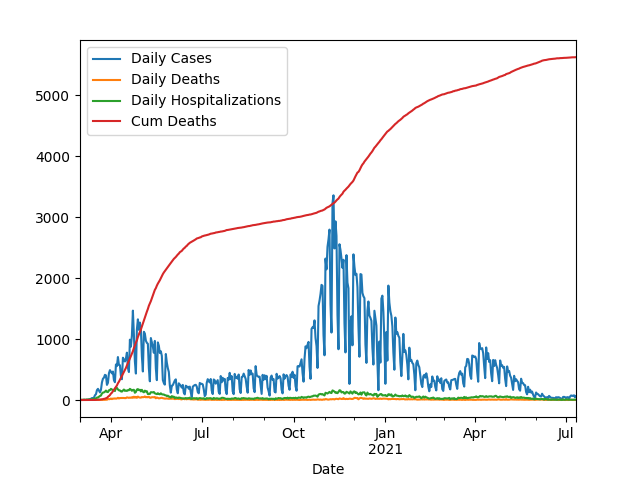
\includegraphics[width=8cm]{series_plot}
		\caption{Reported cases in Chicago.}
		\label{fig:series_plot}
	\end{figure}
	
	\begin{align}
		S_t &= - \beta_{SA} SA - \beta_{SI} SI - \mu S, \\
		E_t &= \beta_{SA} SA - \beta_{SI} - (\sigma_A + \sigma_I) E, \\
		A_t &= \sigma_A E - M_{AR} A, \\
		AR_t &= M_{AR} A, \\
		I_t &= \sigma_I E - MI, \\
		H_t &= \gamma M I - (1 - \omega) \chi H - \omega \psi H, \\
		R_t &= (1 - \gamma) M I + (1 - \omega) \chi H, \\
		D_t &= \omega \psi H.
	\end{align}
	
	We determine the optimal parameters by minimizing the Euclidean distance $\N$ between the time series generated by the model (num) and the corresponding observed time series (obs),
	\begin{equation}
		\N = \sum_i \left( \left| \log(C_{\num}(t_i)) - \log(C_{\obs}(t_i)) \right|^2
		+ \left| \log(D_{\num}(t_i)) - \log(D_{\obs}(t_i)) \right|^2 \right)
	\end{equation}
	where the index $i$ identifies a point in the time series.
	The optimization tries to reproduce the number of total reported cases ($C(t) = I(t) + H(t) + R(t) + D(t)$) and the total number of deceased ($D(t)$). \cite{Kevrekidis_2021}
	
	We can account for a change in the parameters due to the lockdown by imposing a time dependence on the transmission rates $\beta$:
	\begin{align}
		\beta_{IS} (t) &= \beta_{IS} \left[ \eta_{IS} + (1 - \eta_{IS}) \frac{1 - \tanh[2(t - t_q)]}{2} \right], \\
		\beta_{AS} (t) &= \beta_{AS} \left[ \eta_{AS} + (1 - \eta_{AS}) \frac{1 - \tanh[2(t - t_q)]}{2} \right].
	\end{align}
	This causes the transmission rates $\beta_{IS}$ and $\beta_{AS}$ to decrease abruptly by a factor of $\eta_{IS}$ and $\eta_{AS}$ respectively at the time $t_q$ when the lockdown was imposed. \cite{Wang_2020}
	
	\begin{center}
	\begin{tabular}{ c c c c c }
		\hline
		\hline
			&	&	Median ($t_q = 3$)	&	Median ($t_q = 16$)	&	Initial value \\
		\hline
		Population	&	$N$	&	\multicolumn{3}{ c }{2,693,976} \\
		Initial populations & $(I_0, H_0, D_0)$	&	\multicolumn{3}{ c }{$(297, 134, 6)$} \\
		Non COVID-19 death rate [per day]	&	$\mu$	&	\multicolumn{3}{ c }{$5.79 \times 10^{-7}$} \\
		Transmission rate, $S \rightarrow I$ [per day]	&	$\beta_{IS}$	&	$0.35 (0.28-0.41)$	&	$0.32 (0.29-0.35)$	&	$c \in U[0,1]$ \\
		\hline
		\hline
	\end{tabular}
	\end{center}

\bibliographystyle{siam}
\bibliography{chicago-spatial-covid}

\end{document}